\subsection{Solenoid and Torus Magnets}


\subsubsection{Geometry}
The solenoid geometry is produced with the GEMC perl API. The solenoid is a single polycone volume, shown in \F{solenoid}.
\begin{figure}[h]
	\centering
	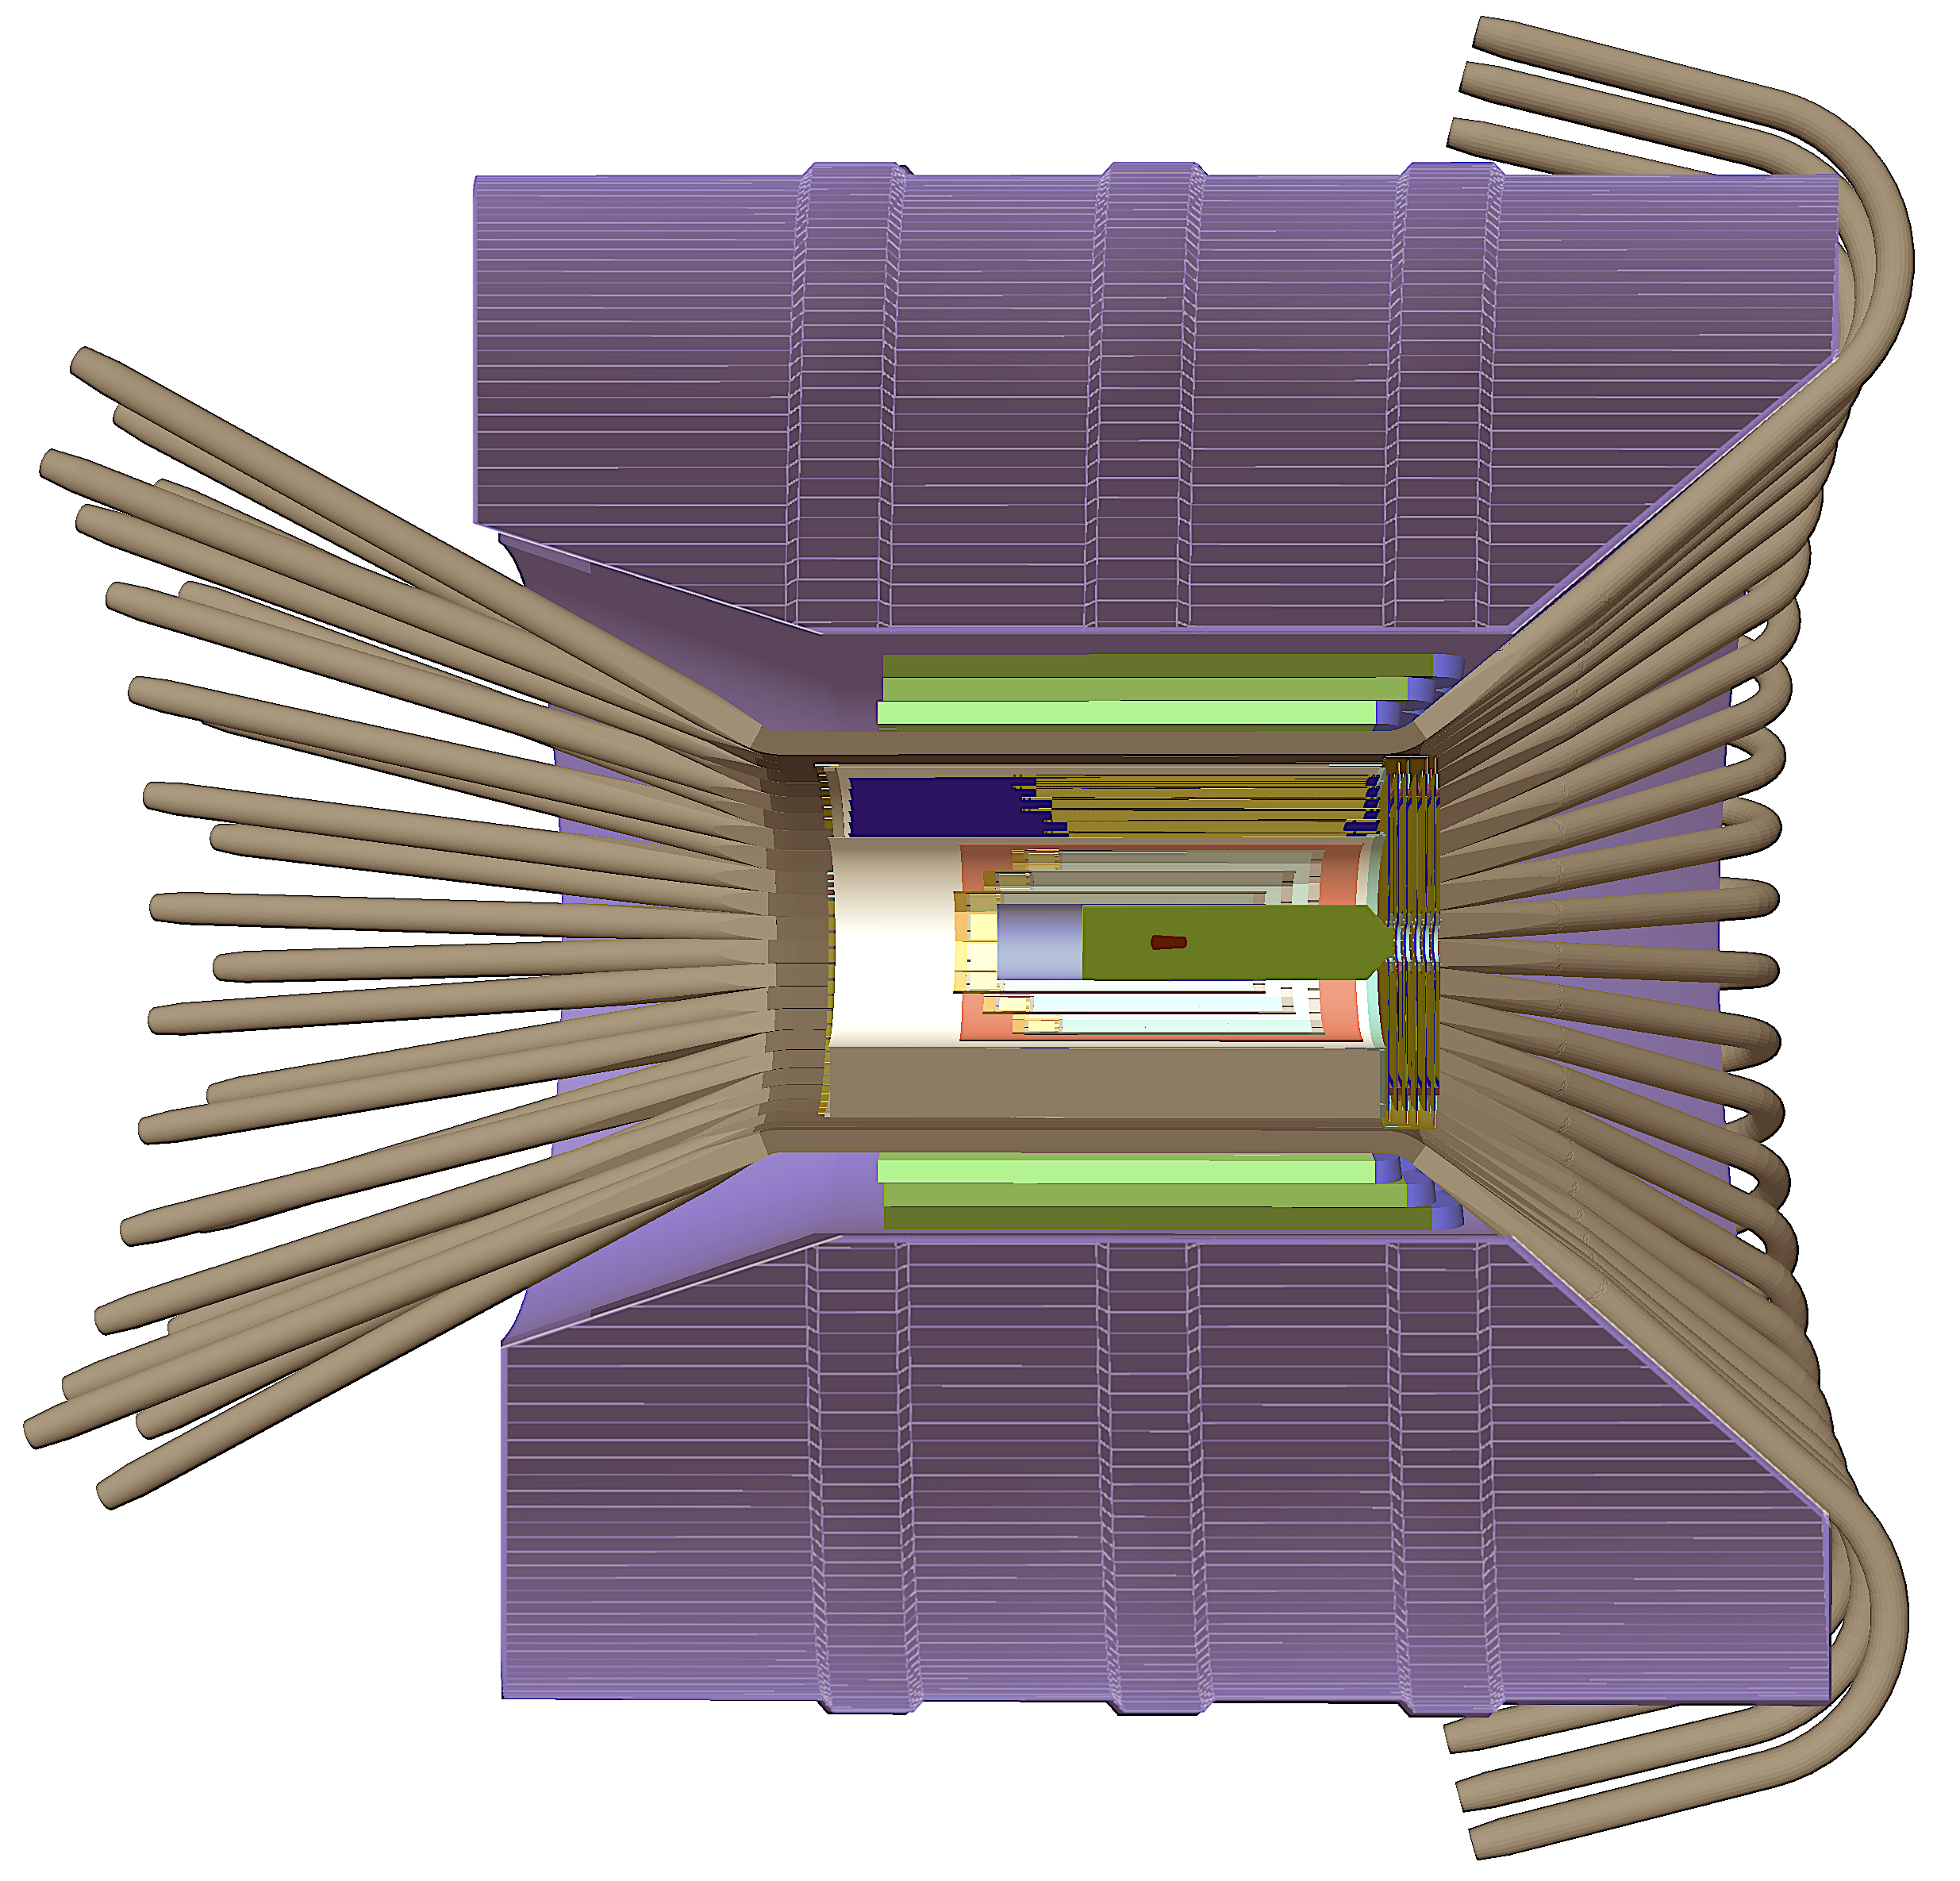
\includegraphics[width=0.99\columnwidth,keepaspectratio]{img/solenoid.png}
    \caption{The solenoid volume surrounding the CLAS12 Central Detector.}
	\label{fig:solenoid}
\end{figure}

The torus geometry is imported from the engineering CAD model through 54 tessellated volumes. Among the volumes are:

\begin{itemize}
	\item the bore heat shield and hub components
	\item the back and front hub steel plates
	\item the stainless steel coil vacuum jackets
	\item the torus coils containing the conductors, represented by copper volumes in Geant4
	\item internal shielding around the hub, made by tungsten cylinders (blue in \F{torus})
\end{itemize}

The torus hub is protected from the beampipe background with additional tungsten shielding.
The torus geometry is shown in \F{torus}.

\begin{figure}
	\centering
	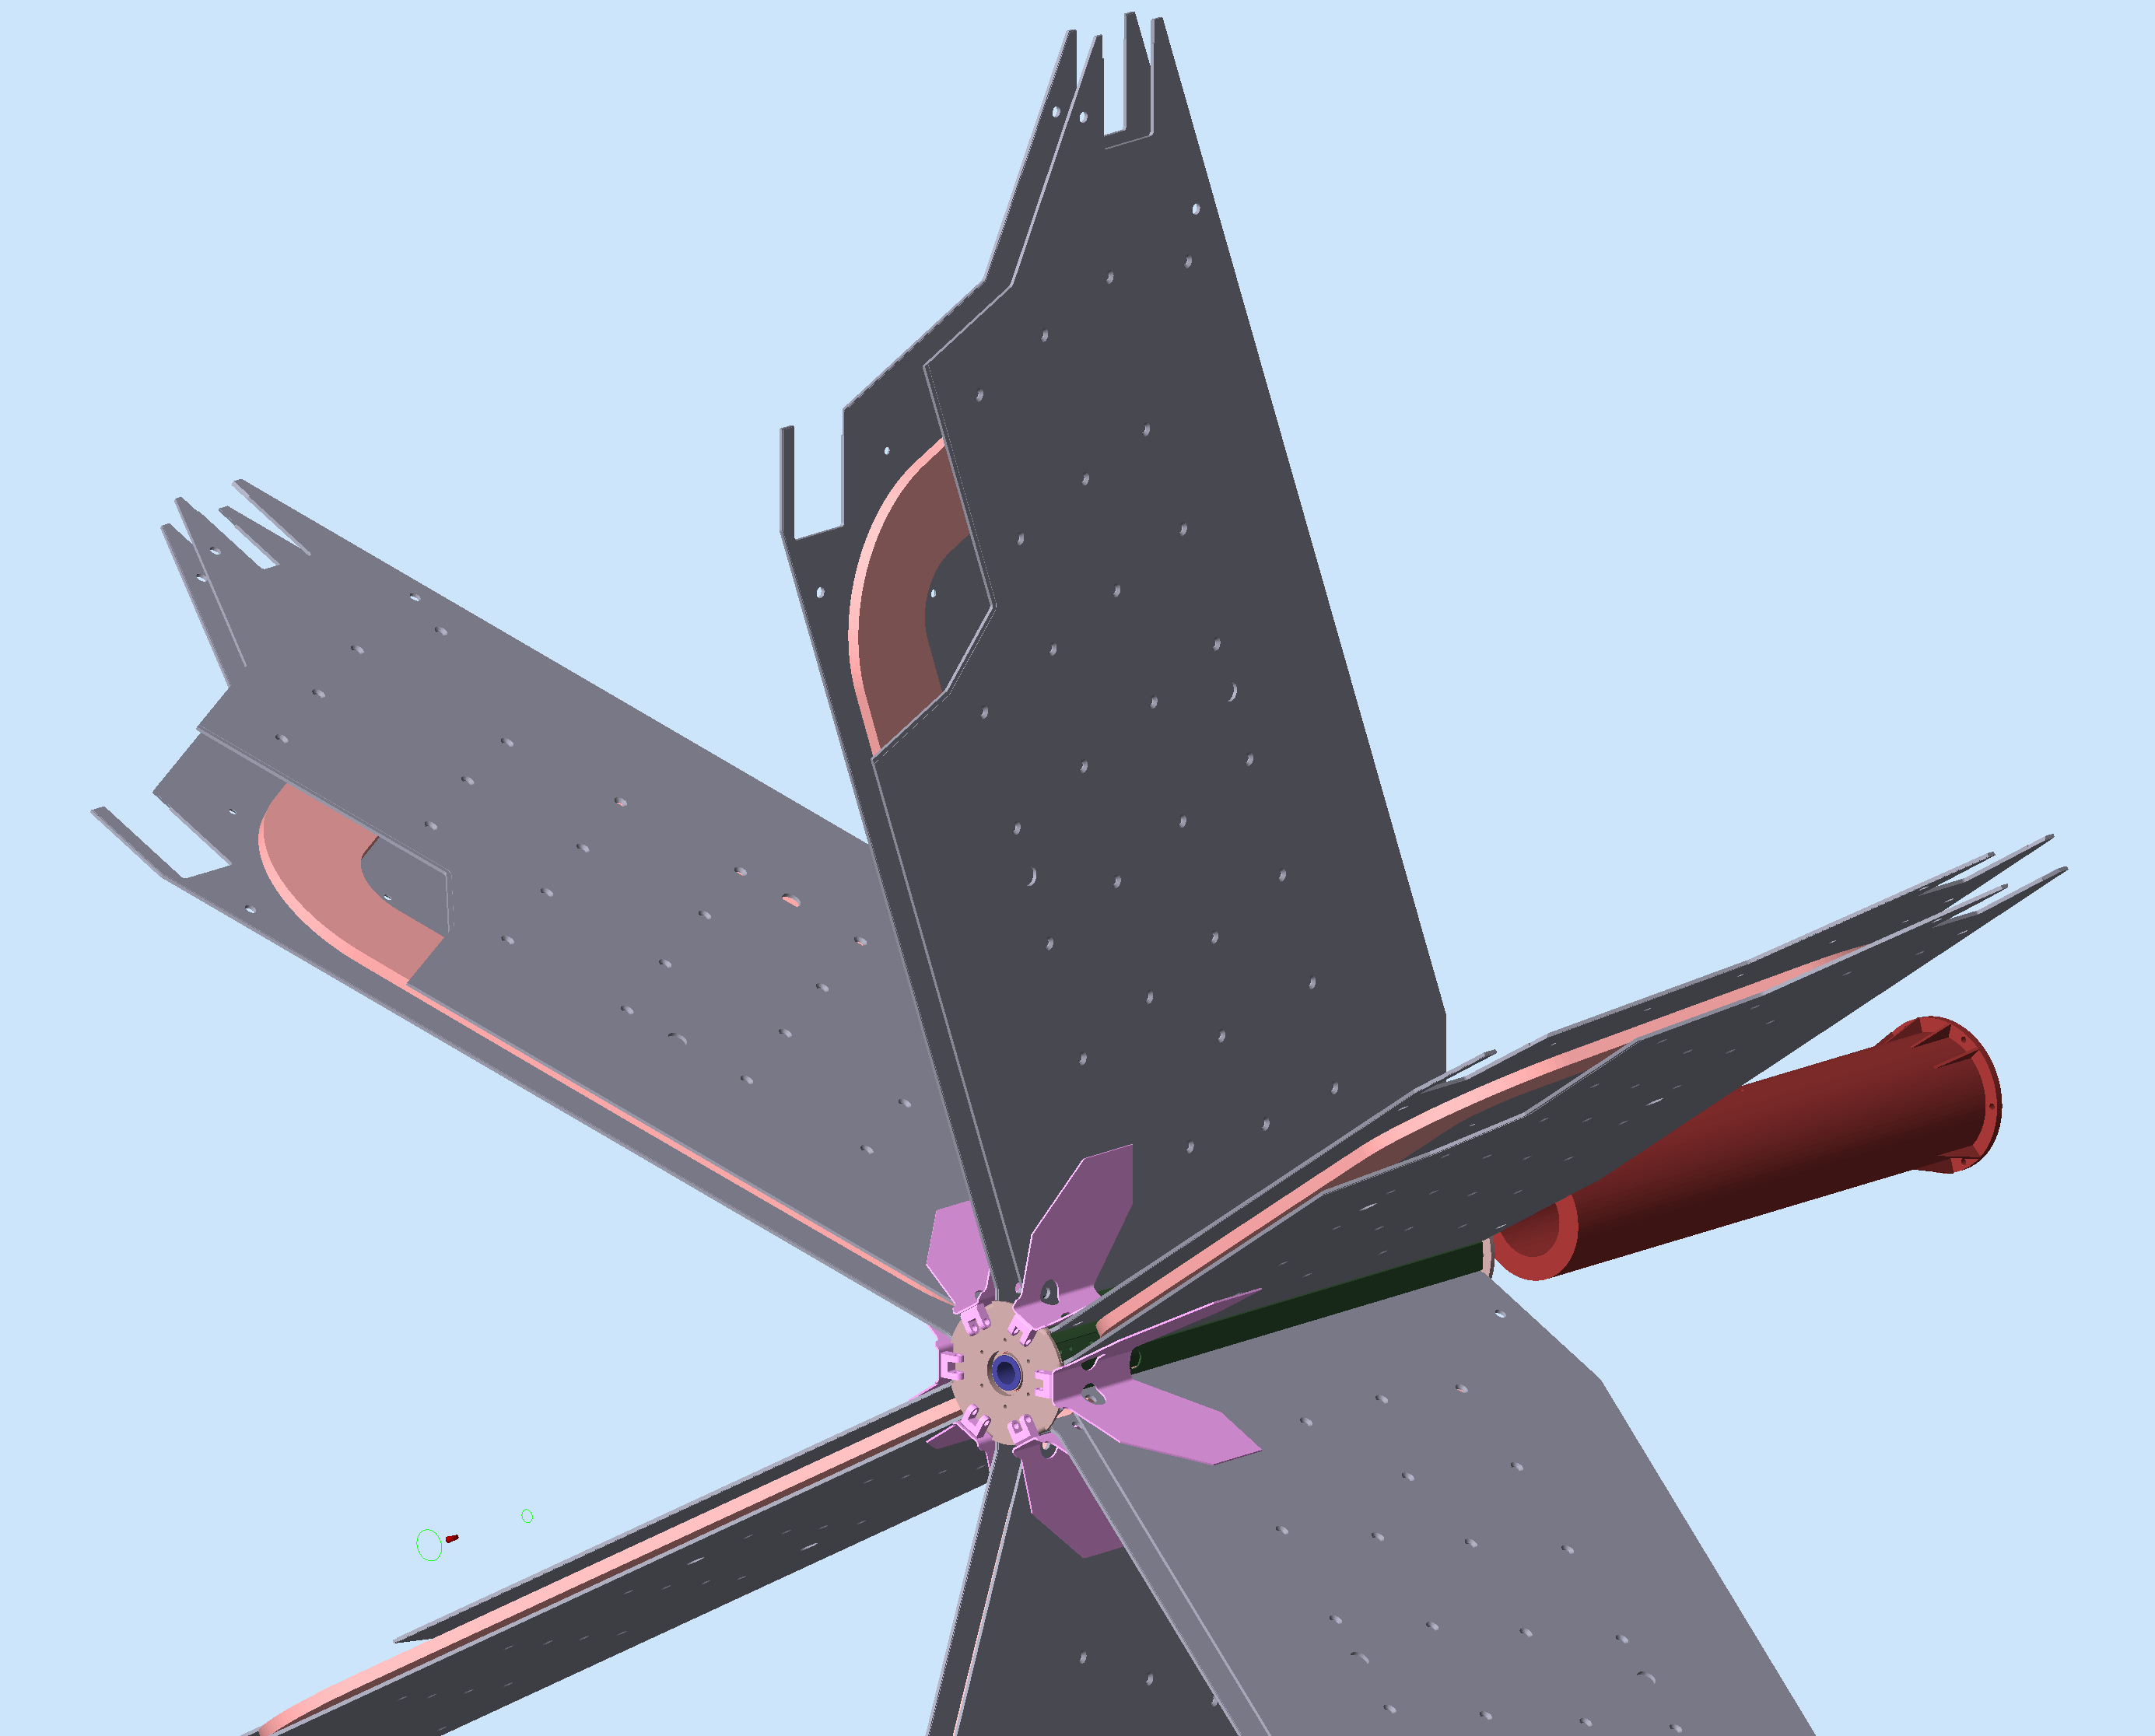
\includegraphics[width=0.99\columnwidth,keepaspectratio]{img/torusGeometry.png}
	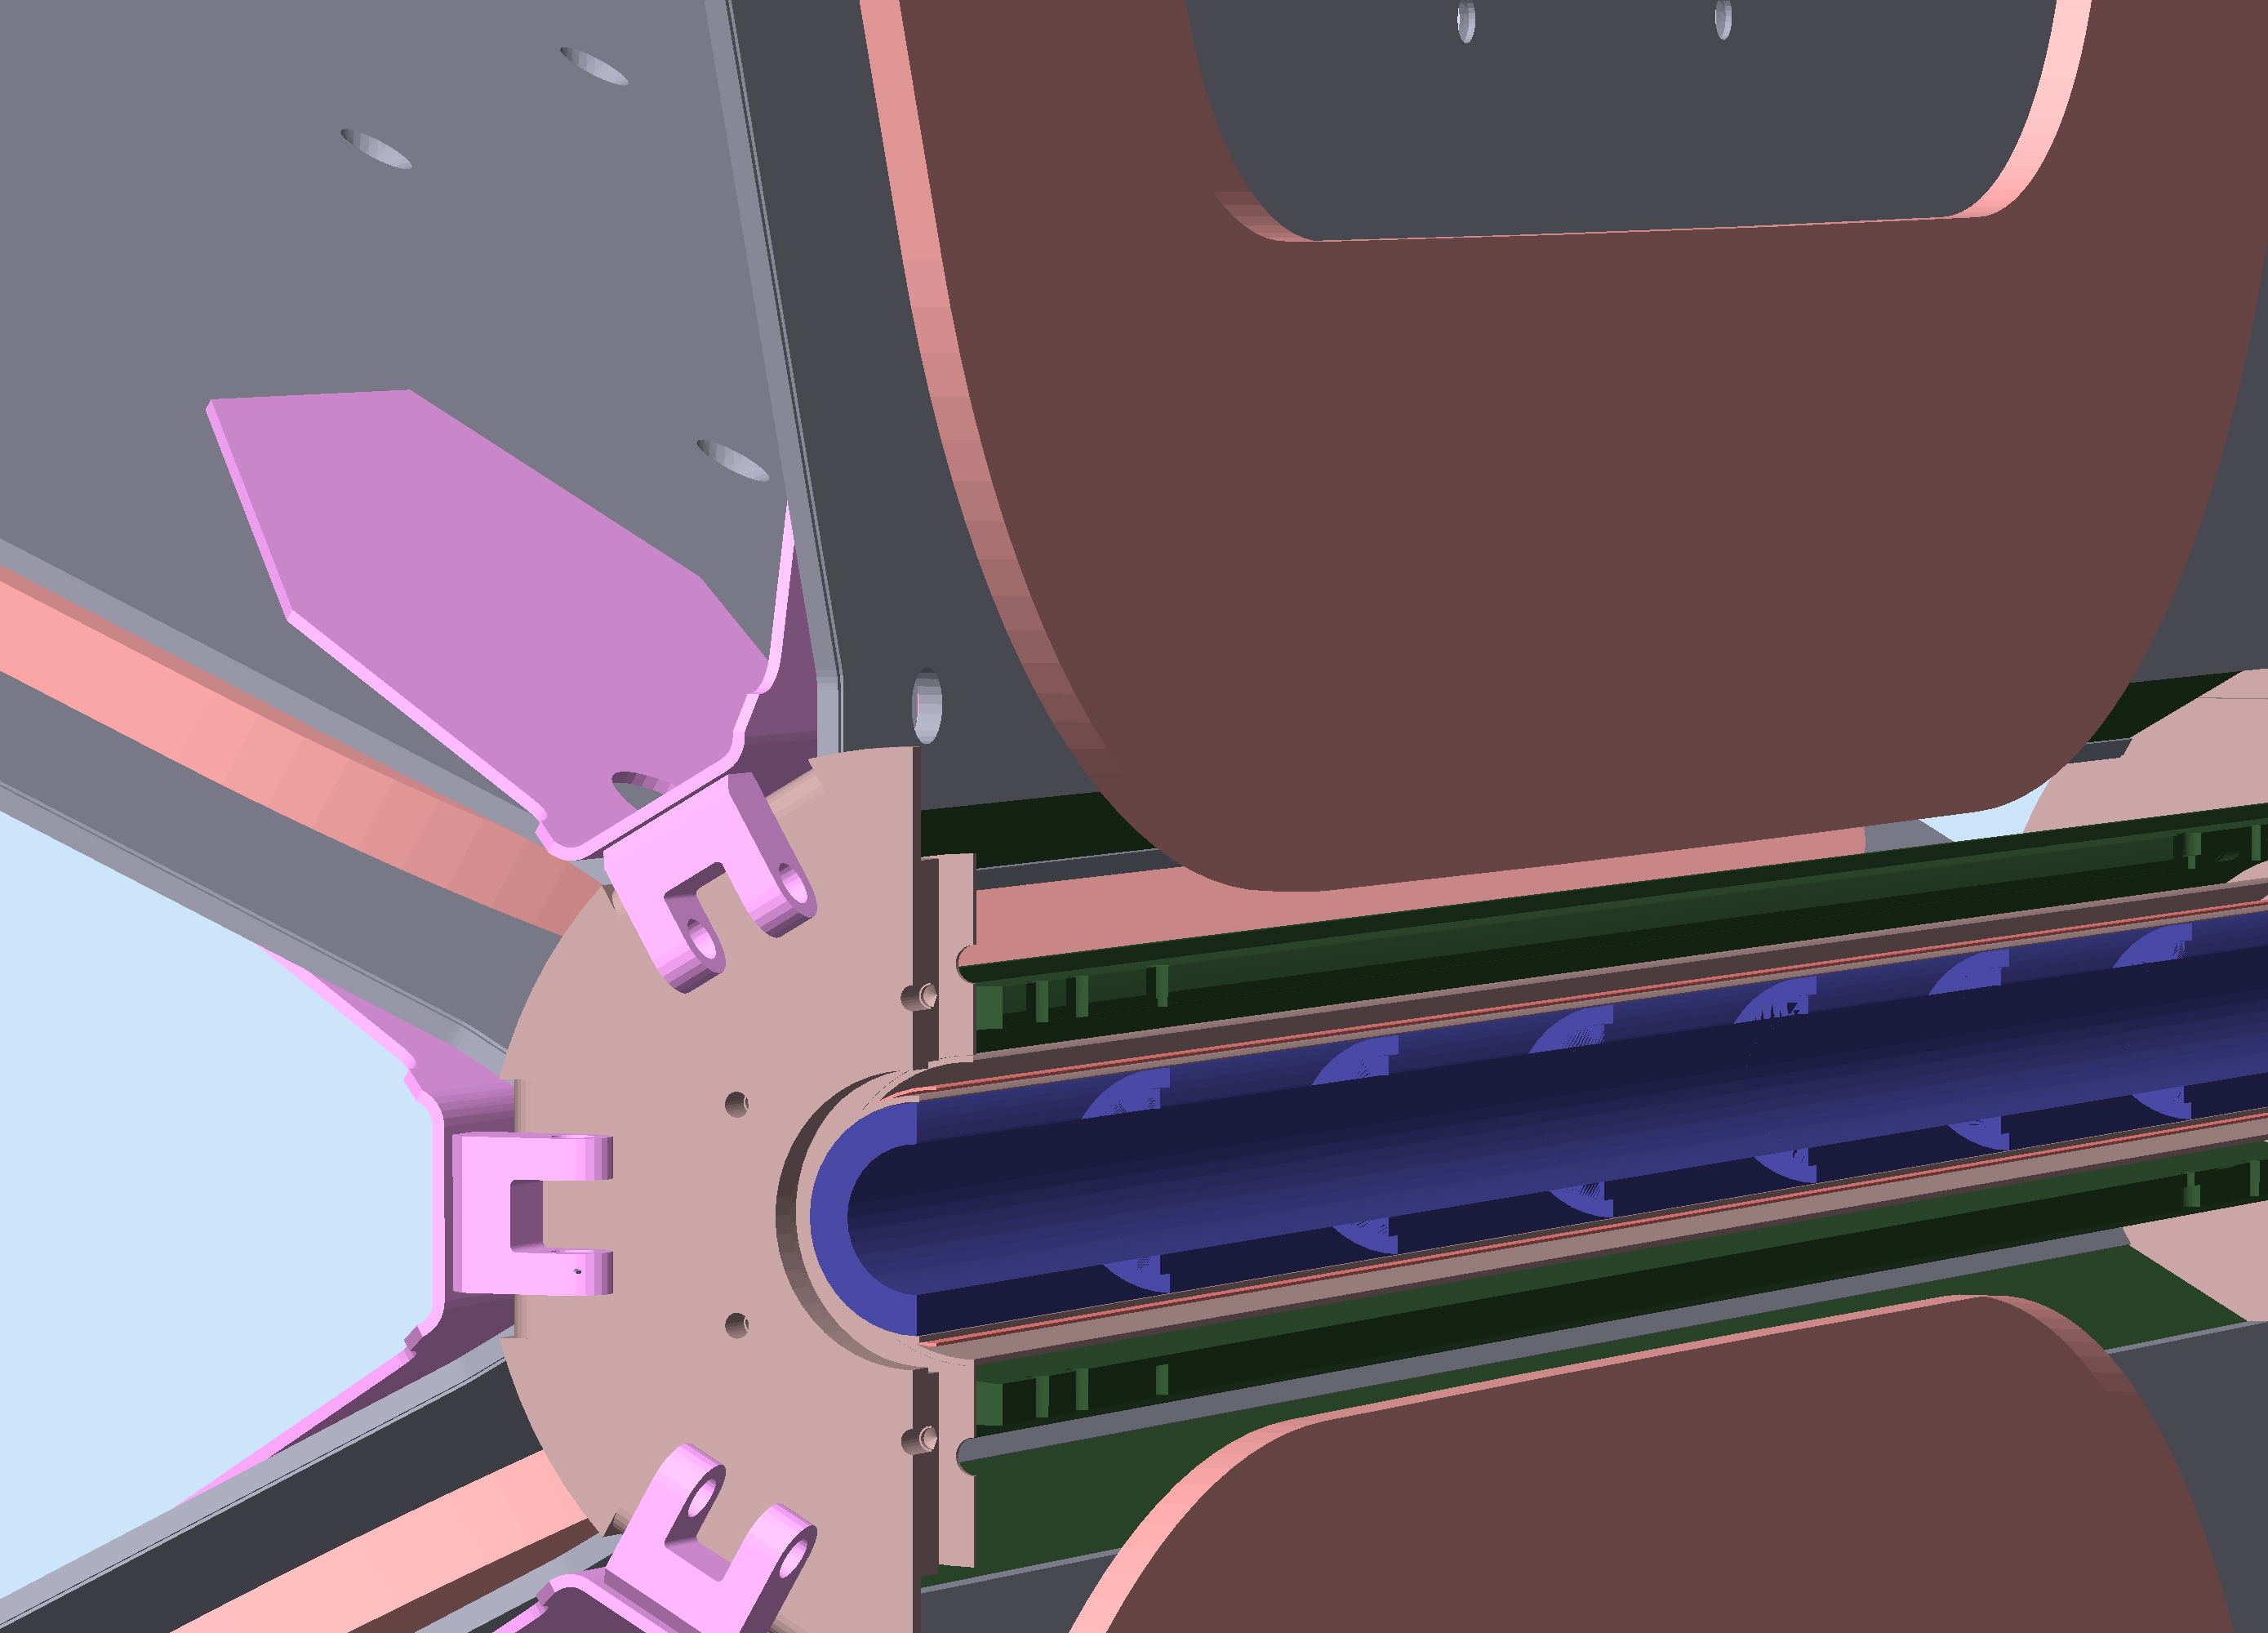
\includegraphics[width=0.99\columnwidth,keepaspectratio]{img/torusDetail.png}
	\caption{Top: the GEMC implementation of the torus hardware. The volumes are imported from the CAD engineering model.
             The stainless steel vacuum jacket embeds the Geant4 coil volumes.
			 Bottom: a section view of the torus in the vicinity of the beamline. The warm and cold hubs are visible, along with the
			 tungsten shielding in the innermost part of the hub.}
	\label{fig:torus}
\end{figure}


\subsubsection{Magnetic Field Maps} \label{sec:clas12FieldMaps}

The CLAS12 torus and solenoid field maps are imported into the simulation using ascii files. Both fields can be scaled by an arbitrary factor.
Both fields are defined in the Hall-B coordinate system and both can be shifted and tilted by additional delta amounts.

\subsubsection{Solenoid}
The solenoid field map has cylindrical symmetry around the $z$-axis, so the map used in the simulation is defined
in the transverse / longitudinal plane and then rotated when requested by the Geant4 navigation.
The integration method used in the simulation is the fourth order Runge-Kutta technique \cite{rungeKutta}.

The solenoid field near the target is parallel to the $z$-axis and its uniformity was measured to be 318 ppm over a 25 mm
diameter and 40 mm long cylindrical volume. The field map grid is made by 600 points in the transverse coordinate,
from 0 to 3 m and by 1200 points along the $z$-axis, from \mbox{-3 m} to 3 m.
The field grid values are linearly interpolated to the $(x,y,z)$ coordinate requested by Geant4.
Table \ref{tab:solMap} shows the field map ascii data structure. The simulation of one event in a 250 ns time window at
the CLAS12 luminosity with and without solenoid magnetic field is presented in \F{solenoidONOFF}, showing the effectiveness
of the solenoid in providing electromagnetic shielding to M\"oller electrons.

\begin{table}[h]
	\begin{center}
		\begin{tabular}{| c | c | c | c |}
			T (m)  & Z (m) &  $B_T$ (T) & $ B_L (T)$ \\
			\hline
          0.005  &  -0.025 & 0.000013  & 5.000880 \\
          0.005  &  -0.020 & 0.000044  & 5.000822 \\
          0.005  &  -0.015 & 0.000073  & 5.000704 \\
          0.005  &  -0.010 & 0.000101  & 5.000529 \\
          0.010  &  -0.025 & 0.000028  & 5.000928 \\
          0.010  &  -0.020 & 0.000089  & 5.000867 \\
          0.010  &  -0.015 & 0.000148  & 5.000747 \\
          0.010  &  -0.010 & 0.000203  & 5.000570 \\
		\end{tabular}
	\end{center}
\caption{Solenoid ascii field map values around the target. T is the transverse coordinate $\sqrt{(x^2+y^2)}$ and $z$ is the longitudinal coordinate.
		 The solenoid field is centered at $z=0$, the location of the center of the target.}\label{tab:solMap}
\end{table}

\begin{figure}
	\centering
	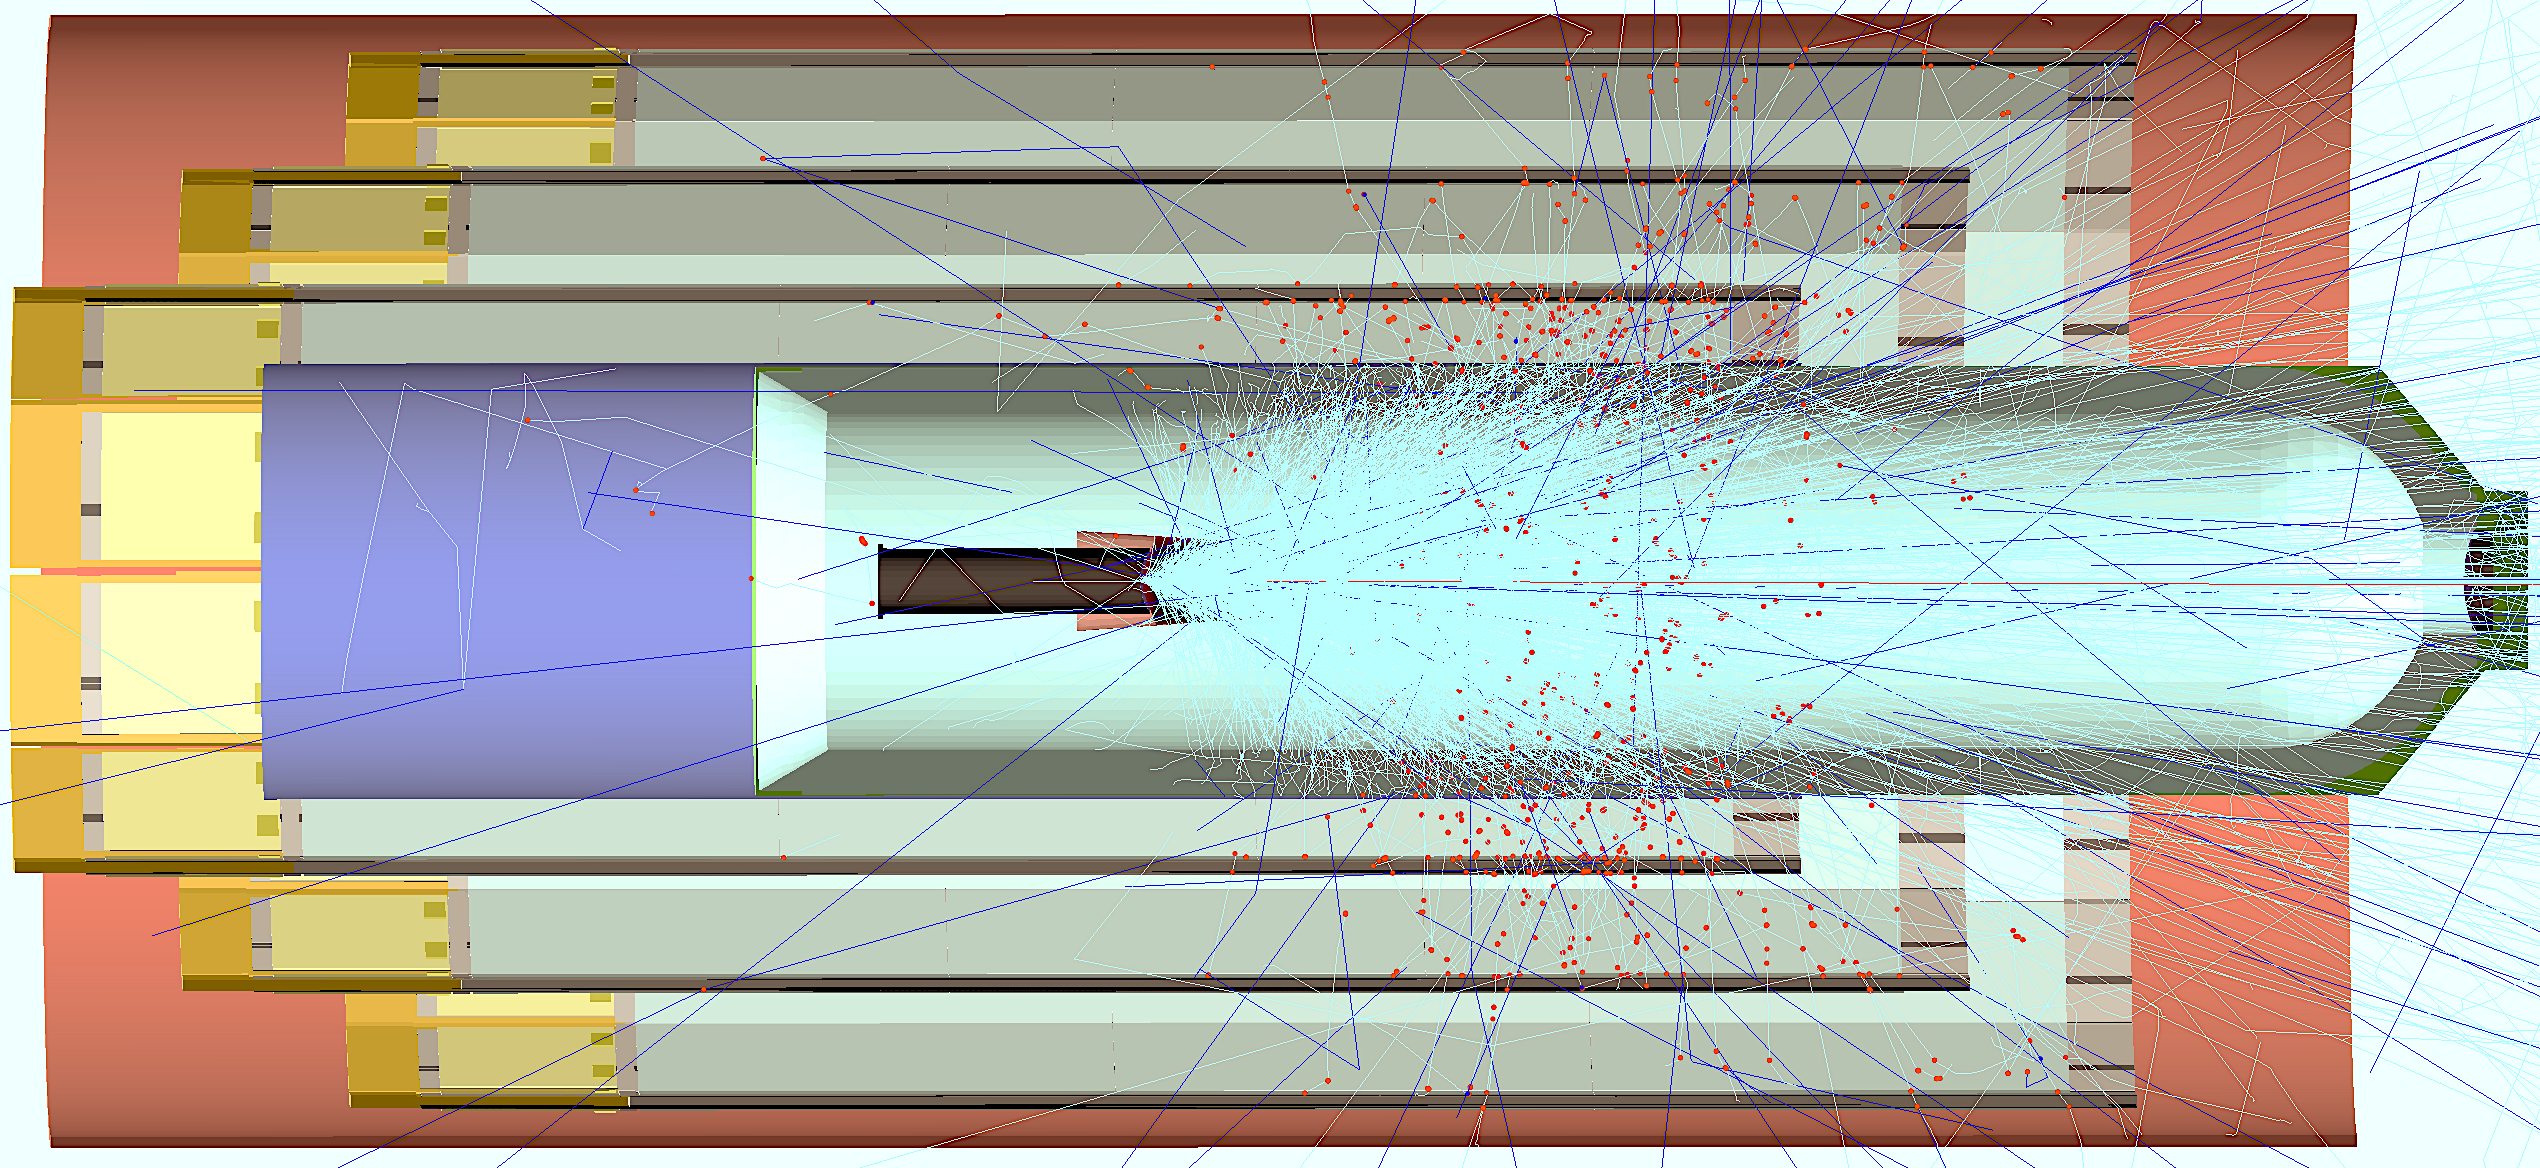
\includegraphics[width=0.98\columnwidth,keepaspectratio]{img/solenoidOFF.png}
	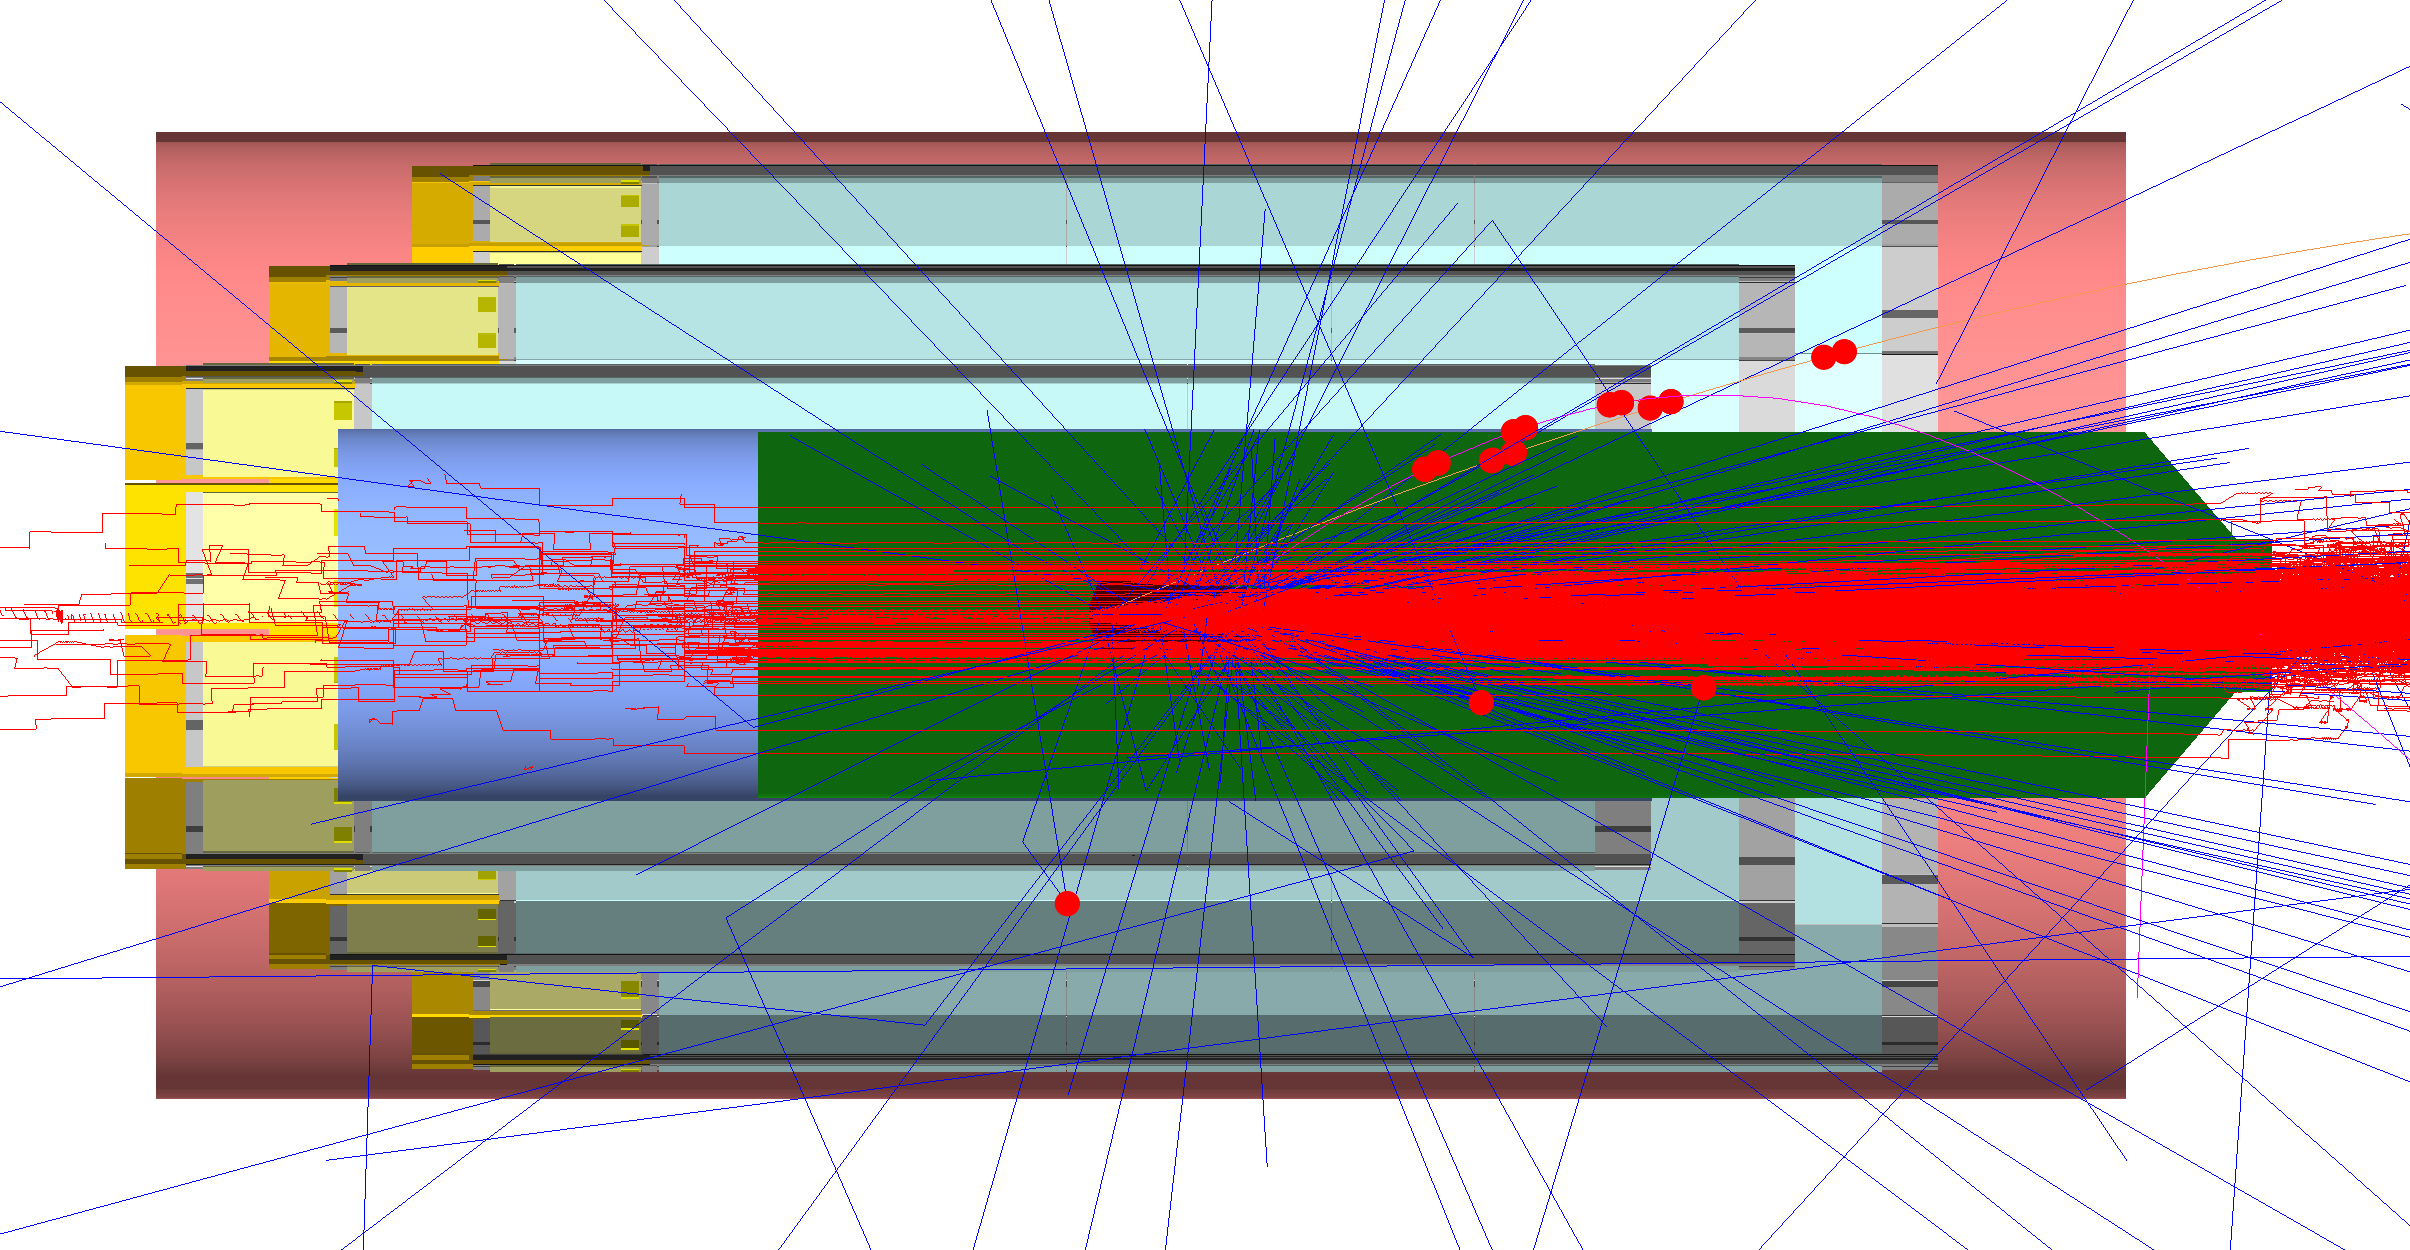
\includegraphics[width=0.98\columnwidth,keepaspectratio]{img/solenoidON.png}
    \caption{An 11 GeV electron beam impinges on a 5-cm long liquid-hydrogen target. The SVT detector is shown.
             At the full 10$^{35}$ cm$^{-2}$ s$^{-1}$ luminosity, this correspond to 124,000 electrons in a 250 ns time window.
			 Top: no solenoid field. One full luminosity event in a 250 ns time window produce a storm of M\"oeller electrons that
             saturates the SVT. Each red point is a recorded hit above the SVT threshold.
			 Bottom: full solenoid field. One full luminosity event in a 250 ns time window.
             The solenoid focuses all of the M\"oeller electrons along the beamline, providing an effective electromagnetic shield for CLAS12.
			 The only hits above threshold are the ones generated by real hadronic tracks. }
	\label{fig:solenoidONOFF}
\end{figure}

\subsubsection{Torus}
The torus field can be imported using a symmetric map or a full 3D map.
The symmetric map is defined in half of a CLAS12 sector. It is symmetric around the sector mid-plane and copied in each sector
when requested by the Geant4 navigation. The 3D map covers the entire cartesian space and accounts for field deviations due to coil
movements or imperfections \cite{GhoshalSolenoid}.

The field map has 251 points along the $z$-axis, from 1 m to 3 m. It has 2501 points in the transverse coordinate, from 0 to 5 m.
It has 16 azimuthal points from 0\mdeg to 30\mdeg. The field grid values are linearly interpolated to the $(x,y,z)$
coordinate requested by Geant4.

The torus field in the sector mid-plane is perpendicular to the $z$-axis and is typically $2.058$ T.
Table \ref{tab:torMap} shows the field map ascii data structure.

\begin{table}[h]
	\begin{center}
		\begin{tabular}{| c | c | c | c | c | c | }
         $\phi$ (deg) & T (m)    & Z (m)    &  $B_x$  &    $B_y (T)$    & $B_z$\\
			\hline
          0.0         &  190.0   &  338.0   &  0       &     0.451275 &  0 \\
          0.0         &  190.0   &  340.0   &  0       &     0.450136 &  0 \\
          0.0         &  190.0   &  342.0   &  0       &     0.448789 &  0 \\
          0.0         &  190.0   &  344.0   &  0       &     0.447235 &  0 \\
          0.0         &  190.0   &  346.0   &  0       &     0.445472 &  0 \\
          0.0         &  190.0   &  348.0   &  0       &     0.443502 &  0 \\
          0.0         &  190.0   &  350.0   &  0       &     0.441323 &  0 \\
          0.0         &  190.0   &  352.0   &  0       &     0.438935 &  0 \\
		\end{tabular}
	\end{center}
	\caption{Torus ascii field map values near mid-sector. T is the transverse coordinate $\sqrt{(x^2+y^2)}$ and
             $z$ is the longitudinal coordinate.}
 	\label{tab:torMap}
\end{table}


